\documentclass{beamer}
\usepackage{amsmath}
\usepackage{graphicx}
\mode<presentation>
{
  \usetheme{default}
  \usecolortheme{seahorse}
}

\title{Formal Verification of Chained Moonshot SMR Protocol}
\author{ M.~Praveen, Chandradeep Dey, Namratha Reddy
\\ Acknowledging: Isaac Doidge, Raghavendra Ramesh}
\institute{Chennai Mathematical Institute ~\textbar~ Supra Oracles }
\date{November 2023}

\begin{document}
\begin{frame}
    \titlepage
\end{frame}

\begin{frame}
    \frametitle{Goal of the Project}
    \begin{itemize}
        \item Supra Research has invented highly efficient (both in
            terms of throughput and latency) Chained Moonshot State
            Machine Replication protocol. White paper is available on
            Supra website and the academic version will be soon on
            ePrint.
            \pause
            \vfill
        \item The papers contain full safety and liveness proofs, hand
            written by experts.
            \pause
            \vfill
        \item The safety and liveness proofs are written in English
            language, prone to errors and overlooks by humans. Even
            proofs in classical mathematics published in peer reviewed
            journals are known to have errors (subtle, hard to
            detect).
            \pause
            \vfill
        \item In its 1994 annual report, Intel wrote that it incurred a cost of USD 494 million for recalling and replacing defective Pentium processors.
        \pause
        \vfill
        \item Industry has come a long way and now (especially the hardware industry) has made formal verification an integral part of design and development.
    \end{itemize}
\end{frame}

\begin{frame}
\frametitle{Goal of the Project}
\begin{itemize}
        \item There are many ways to do formal verification. One is to write English proofs in a formal language (similar to programming language, but meant for writing proofs) and check it for correctness by running it through a machine proof checker.
        \pause
        \vfill
        \item Formally verifying software is much harder than hardware. But with recent advances, it is becoming the golden standard for giving any kind of assurance.
        \pause
        \vfill
        \item The goal of this project is to write the safety proof of the chained Moonshot SMR protocol in a formal language and check its correctness by automated proof checkers.
        \pause
        \vfill
        \item Extensive testing and peer review do a good job of detecting the presence of bugs, but can still miss subtle ones. Proving the absence of bugs can be done only through formal verification.
    \end{itemize}
\end{frame}

\begin{frame}
    \frametitle{Tools and Methods Used}
    \begin{itemize}
        \item \alert{IVy}: a deductive
            verification tool, verified Tendermint, (part of) HotStuff etc.
            \pause
            \vfill
        \item Moonshot pseudocode $\Rightarrow$ IVy model
            \pause
            \vfill
        \item Desired safety property $\Rightarrow$ IVy invariants
            \pause
            \vfill
        \item Does the model violate the invariants? $\Rightarrow$ Is a set of
            logical formulas satisfiable? \pause $\Rightarrow$ Microsoft Z3
            \pause
            \vfill
        \item Is the set of logical formulas satisfiable? \alert{Yes}:
            an example execution violating the invariant
            \pause
            \vfill
        \item Is the set of logical formulas satisfiable? \alert{No}:
            protocol is safe
            \pause
            \vfill
        \item Main challenge: Z3 can get stuck for hours without
            saying yes or no. \pause Need to know logic to overcome
            this
            \pause
            \vfill
        \item It is an intense and laborious process, needing expertise in both the protocol and logical theory underlying the proof system.\pause Tendermint and similar protocols that have been formally verified are simpler compared to chained Moonshot. This is the first time that an industrial strength protocol as complicated as chained Moonshot has been formally verified
    \end{itemize}
\end{frame}

\begin{frame}
    \frametitle{Artefacts of the project}
     https://github.com/Entropy-Foundation/suprabft-fv/tree/master/suprabft    

     \alert{moonshot.ivy} - Moonshot pseudocode written in IVy
     language\\
     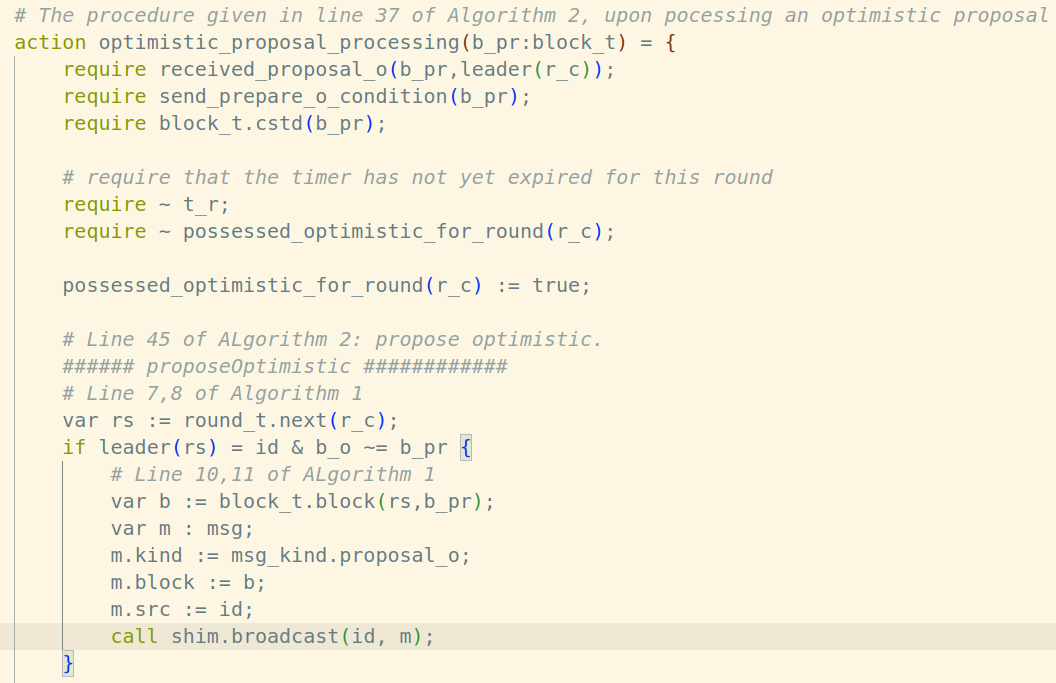
\includegraphics[scale=0.25]{OptimisticPropProc.png}
\end{frame}

\begin{frame}
    \frametitle{Artefacts of the project}
    \alert{quorum\textunderscore{}verification.ivy} - IVy shortcut
    for cryptographic checks of quorum certificates
    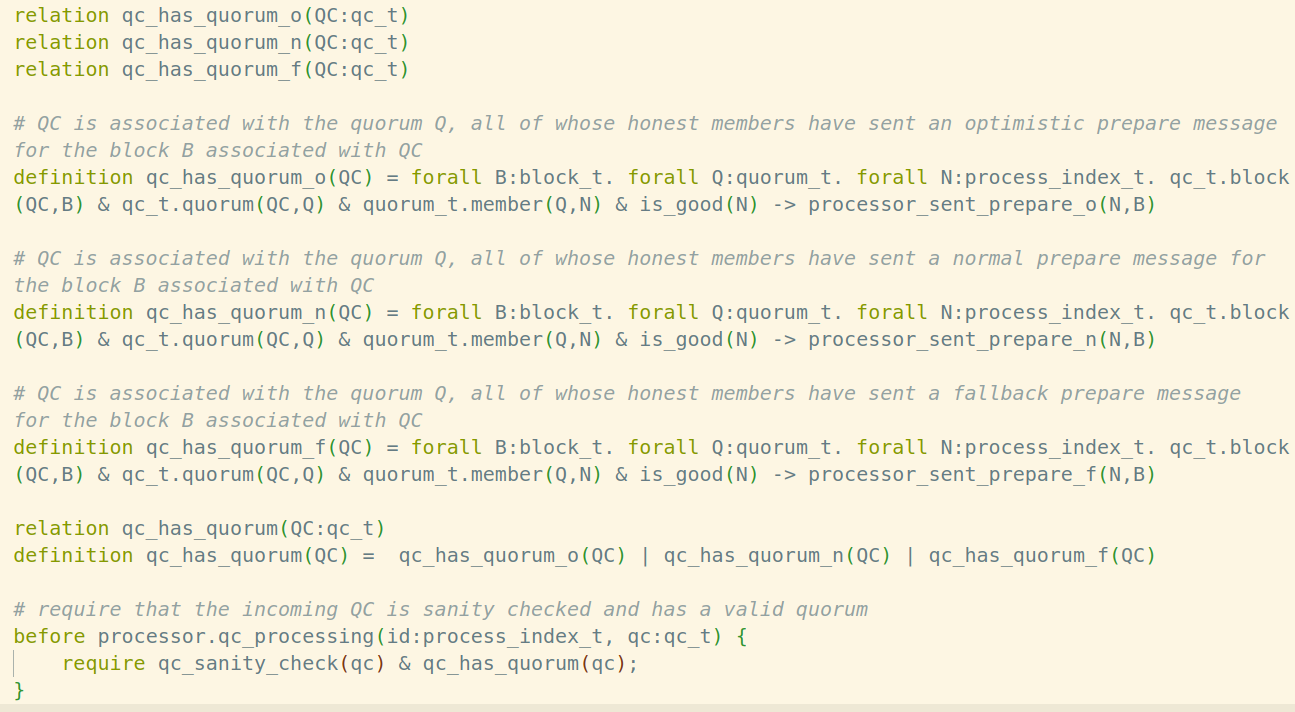
\includegraphics[scale=0.25]{QuorumDef.png}
\end{frame}

\begin{frame}
    \frametitle{Artefacts of the project}
    \alert{safety.ivy} - properties to be verified
    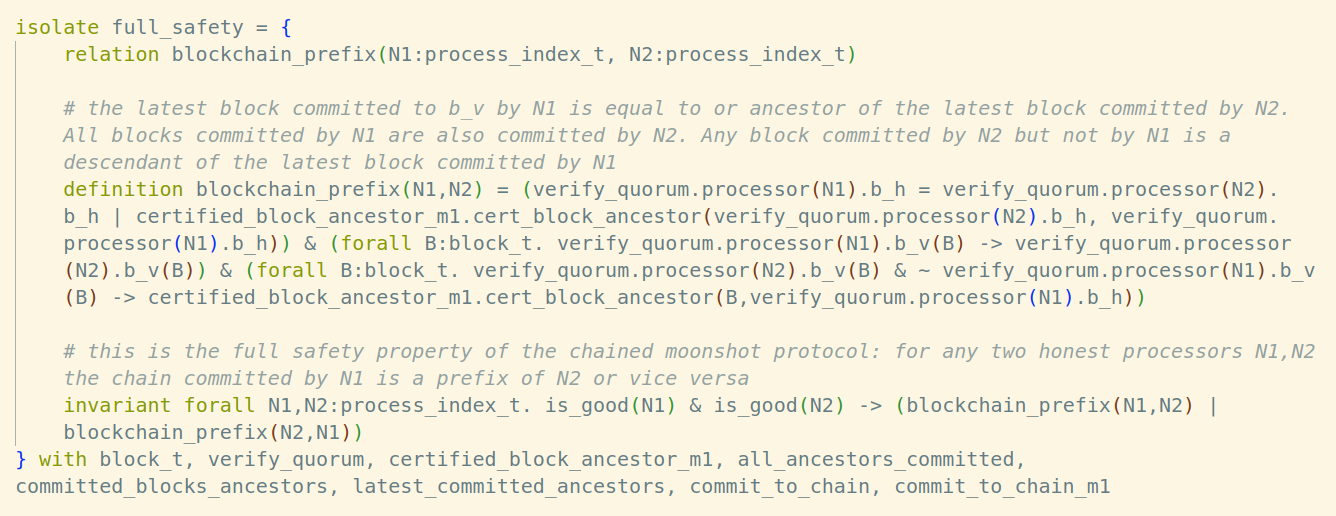
\includegraphics[scale=0.25]{FullSafety.png}
\end{frame}

\begin{frame}
    \frametitle{Byzantine nodes}
    They can send any kind of message to anybody, posing as any other
    Byzantine node
    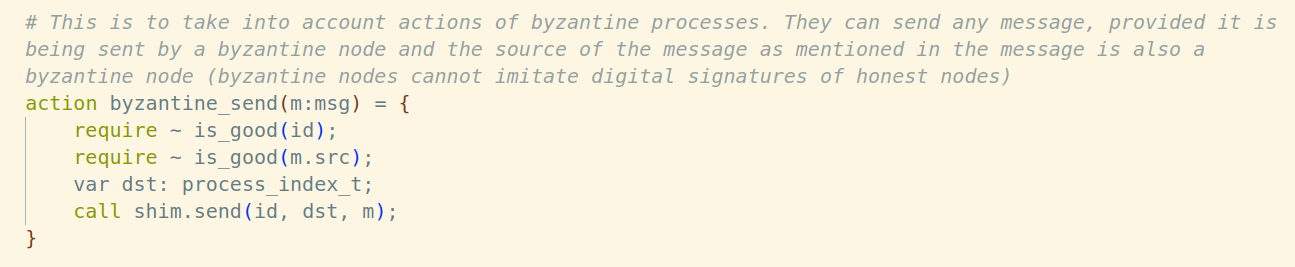
\includegraphics[scale=0.25]{ByzantineSendMsg.png}
    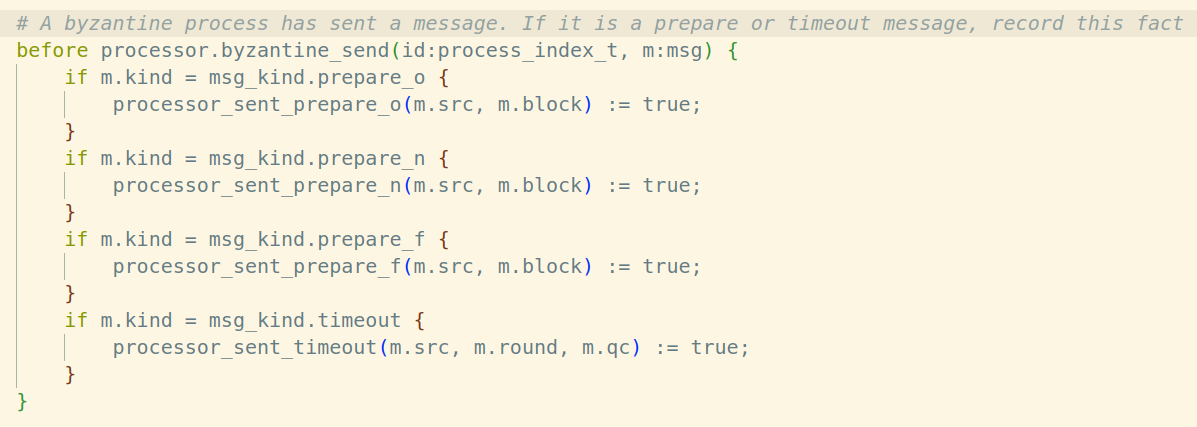
\includegraphics[scale=0.25]{RecordByzantineAction.png}
\end{frame}

\begin{frame}
    \frametitle{Every Minute Detail is Checked}
    Example - If an honest processor votes for a block B, B's parent
    Bp has a lesser round
    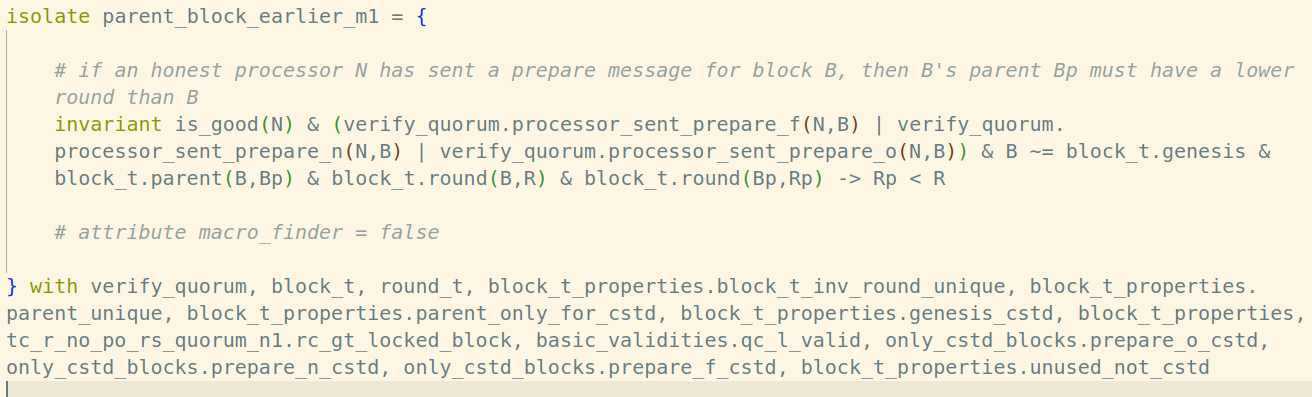
\includegraphics[scale=0.25]{ParentBlockEarlier.png}
    \pause
    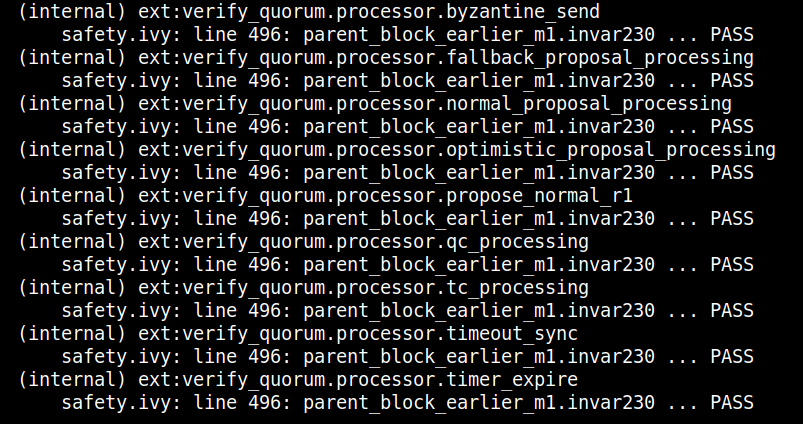
\includegraphics[scale=0.25]{ParentBlockEarlierPass.png}
\end{frame}

\begin{frame}
    \frametitle{Every Minute Detail is Checked}
    Depends on another property: while processing fallback proposals,
    all the QC's in the TC are processed first, so that the current
    round 
    r\textunderscore{}c is strictly greater
    than maxQC of the TC 
    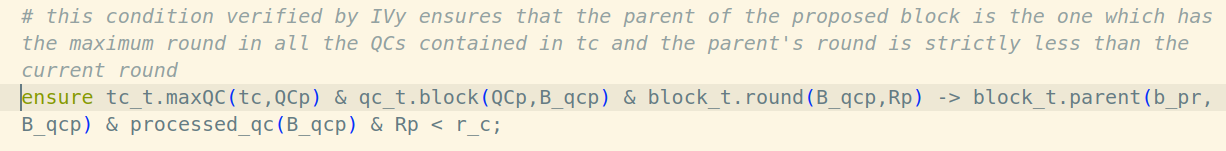
\includegraphics[scale=0.25]{RcGtMaxQC.png}
    \pause
    Suppose we omit the other property
    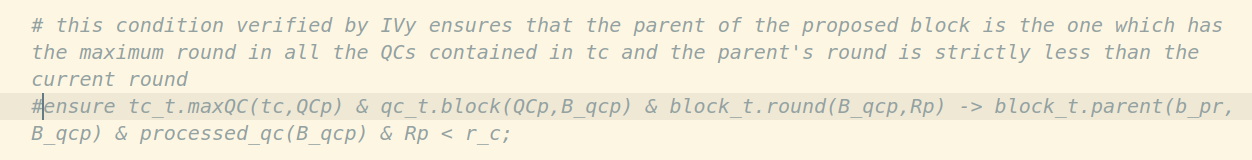
\includegraphics[scale=0.25]{RcGtMaxQCOmit.png}
    \pause
    IVy gives a counter example - block B of round 1 can have parent
    block Bp of round 2
    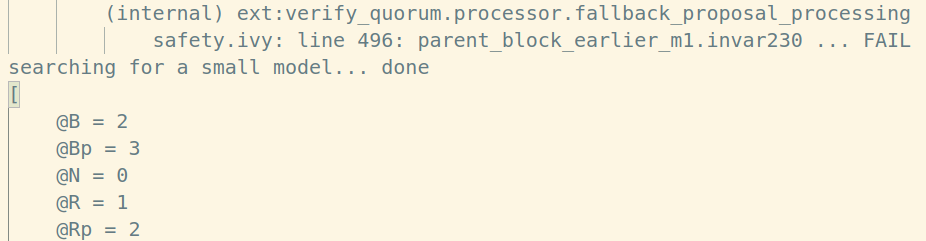
\includegraphics[scale=0.25]{ParentBlockEarlierViolated.png}
\end{frame}

\begin{frame}
    \frametitle{Structure of the safety proof}
    Follows the structure of the proof from Supra Research teams'
    paper

    Theorem 1 is the full safety, the last invariant in safety.ivy
    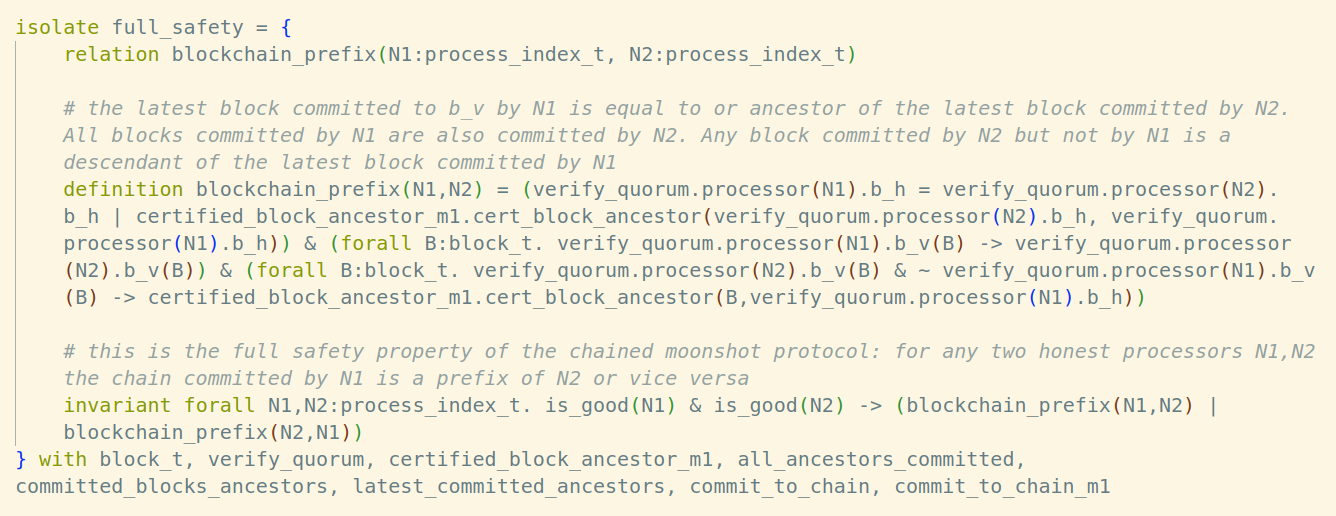
\includegraphics[scale=0.25]{FullSafety.png}
\end{frame}

\begin{frame}
    \frametitle{Structure of the safety proof}

    Depends on Corollary 4, called
    latest\textunderscore{}committed\textunderscore{}ancestors in
    safety.ivy
    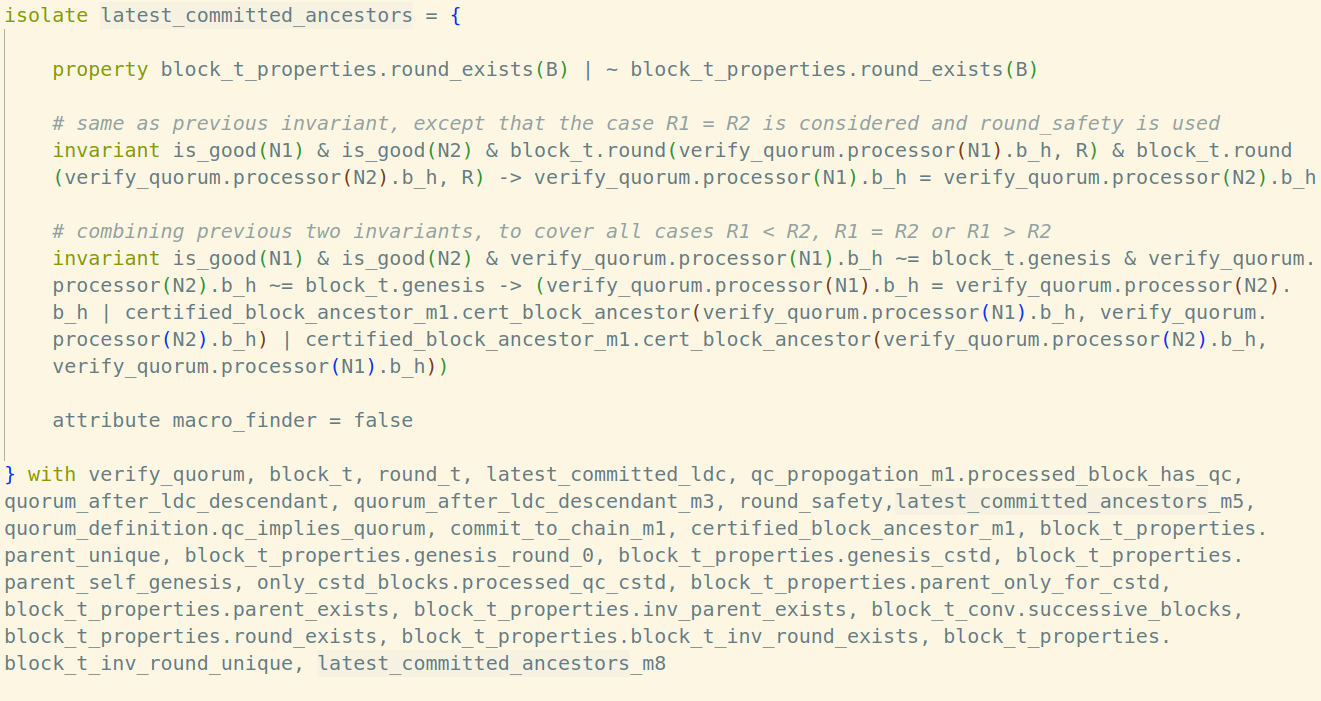
\includegraphics[scale=0.25]{Corollary4.png}

    Proving Corollary 4 is laborious, depends on many other properties
\end{frame}

\begin{frame}
    \frametitle{Structure of the safety proof}
    \begin{itemize}
        \item For proving one invariant, we may need to prove another
            one first \dots
            \pause
            \vfill
        \item Some invariant may be valid, but Z3 gets stuck, so we
            have to logically decompose it into smaller ones for Z3 to
            handle \dots
            \pause
            \vfill
        \item There are totally around 250 invariants that finally
            prove Theorem 1. All are manually written
            \pause
            \vfill
        \item Moonshot has a complicated pipelining mechanism to
            improve latency and throughput. This is the first time a
            such a complicated protocol has been formally verified
    \end{itemize}
\end{frame}
\begin{frame}
    \frametitle{Formal Verification of Commit Moonshot}
    \begin{itemize}
        \item Commit Moonshot is a variant of Chained Moonshot
            protocol
            \pause
            \vfill
        \item After a block is certified, honest processes multicast
            another kind of message called commit message
            \pause
            \vfill
        \item Honest processes commit a block as soon as they receive
            a quorum of commit messages for that block
            \pause
            \vfill
        \item Some parts of the IVy model and invariants from the
            formal verification of chained Moonshot protocol can be
            re-used for the formal verification of commit Moonshot
            protocol. A significant part of the proofs will have to be
            re-worked.
            \pause
            \vfill
        \item A rough estimate is 80 man hours. Formal verification of
            chained Moonshot took 134 man hours after the latest
            round of changes at the end of July.
    \end{itemize}
    \pause
    \vfill
    \begin{center}
        \Large{Thank You}
    \end{center}
\end{frame}
\end{document}
